\section{PID controller validation}
\label{sec:test-1-pid}

% Process of tuning the PIDs
% Graphs from test-controller
% Analysis of error

As mentioned earlier, the person-following mechanism relies on two PID controllers, which serve as the core of the velocity controller. Achieving stable vehicle movement requires tuning the parameters of these controllers to find an appropriate combination.

This section focuses on empirically determining the coefficients for the project's PID controllers. To accomplish this, a dedicated tuning tool, described in Section \ref{subsec:pid-tools} and specifically developed for this purpose, will be utilized. The performance of this tool will be validated using the controller testing tool within the simulated environment, with the flight stack operating in SITL mode. This setup allows for continuous measurement of the PID controllers' response to step movements of a simulated person situated in the 3D world.

Initially, each controller will be independently tuned, enabling the vehicle to move in only one direction at a time. Once the individual tuning is completed, both controllers will be engaged simultaneously to assess their combined response to a variety of inputs. Finally, the complete follow control mechanism will be executed using the obtained tuning parameters to evaluate the final behaviour of the system.

Before calibration, it is necessary to decide on a reference position to set the target values at the controllers. In the world coordinates of the simulated environment, these positions will be x=0 and y=0 for the vehicle and x=600 and y=0 for the person, as depicted in Figure \ref{fig:tune-start-pos}.
From these locations, the person is detected by the vehicles camera centred in the field of view, with a calculated height of 36\% of the image height. Consequently, the controllers running within the simulator will have target set points of 0.5 for the yaw controller and 0.36 for the forward controller.
The result of these target points is that, when the execution starts, for any changes in the position of the person the controllers will transmit velocity commands to the autopilot to achieve the same relative position between the vehicle and the person as between the reference positions.


\begin{figure}[H]
  \centering
  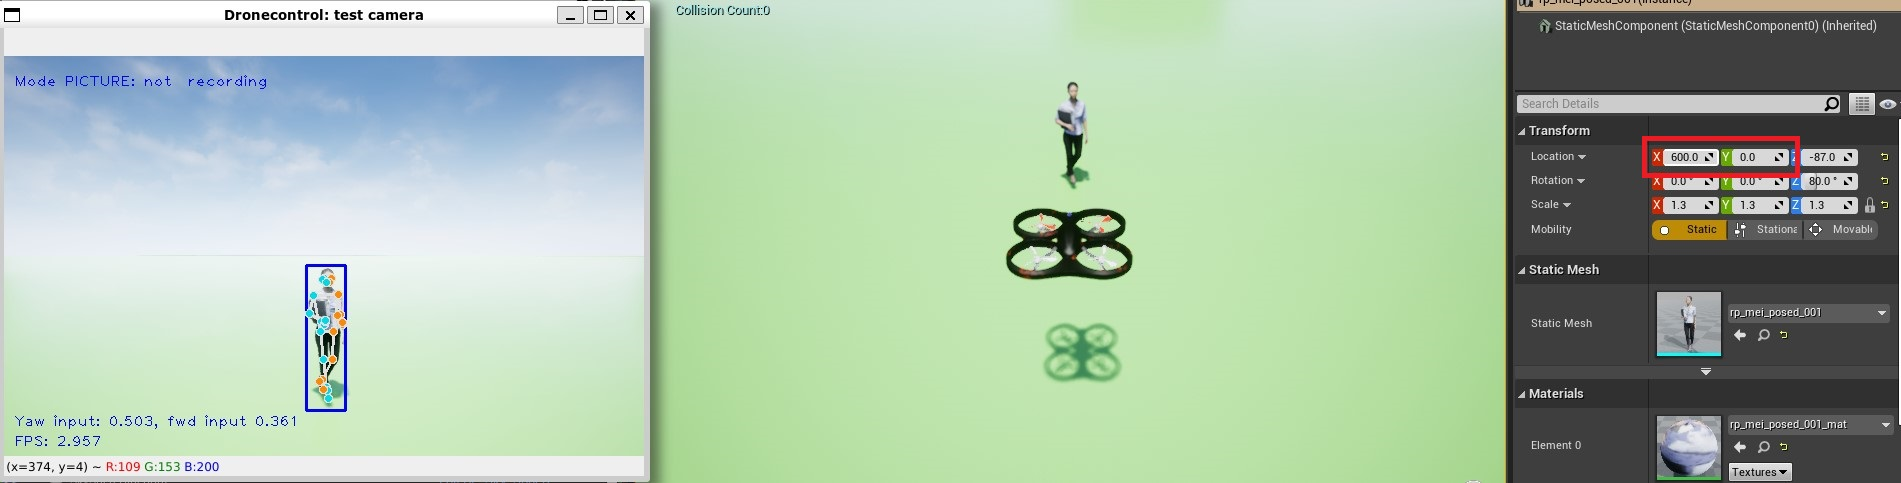
\includegraphics[width=\textwidth, keepaspectratio]{img/pid/tune-ref-pos.jpg}
  \caption{Reference position for the yaw and forward PID controllers. From left to right, the panels show the DroneVisionControl application window, the AirSim simulator world view and the world location of the human model in the simulator. The distance between the vehicle and the person is 600 units in the x direction and 0 units in the y direction.}
  \label{fig:tune-start-pos}
\end{figure}


\subsection{Yaw controller}

To determine the correct coefficients for the controller governing the yaw velocity of the vehicle, the target person is positioned slightly to the side within the field of view. This setup ensures that when the controller is engaged, it outputs a rotation of the vehicle towards that side. Since forward control is not relevant for this test, the target person can be placed closer to the camera to facilitate accurate landmark detection by the pose detection algorithm.

Figure \ref{fig:tune-ref-pos-yaw} illustrates the starting position of the simulated environment before each run. The 3D model representing the person is situated at coordinates (500, 100), which is 100 units to the right of the reference position. In the leftmost panel of Figure \ref{fig:tune-ref-pos-yaw}, the DroneVisionControl application displays an input of 0.62 for the yaw controller at this position. The controller will therefore calculate an error of $\epsilon = 0.5 - 0.62$ (set point minus input) at the start of the test.

The controller must then generate a positive yaw velocity to centre the person within its field of view. With a starting offset position to the right, the error is less than zero. However, a positive velocity is required to counteract this error and induce a rightward yaw velocity. Therefore, the coefficients for the yaw controller need to be negative. This ensures that an increased horizontal position results in a positive yaw velocity to decrease it, as indicated by Equation \ref{eq:pid}.


\begin{figure}[H]
  \centering
  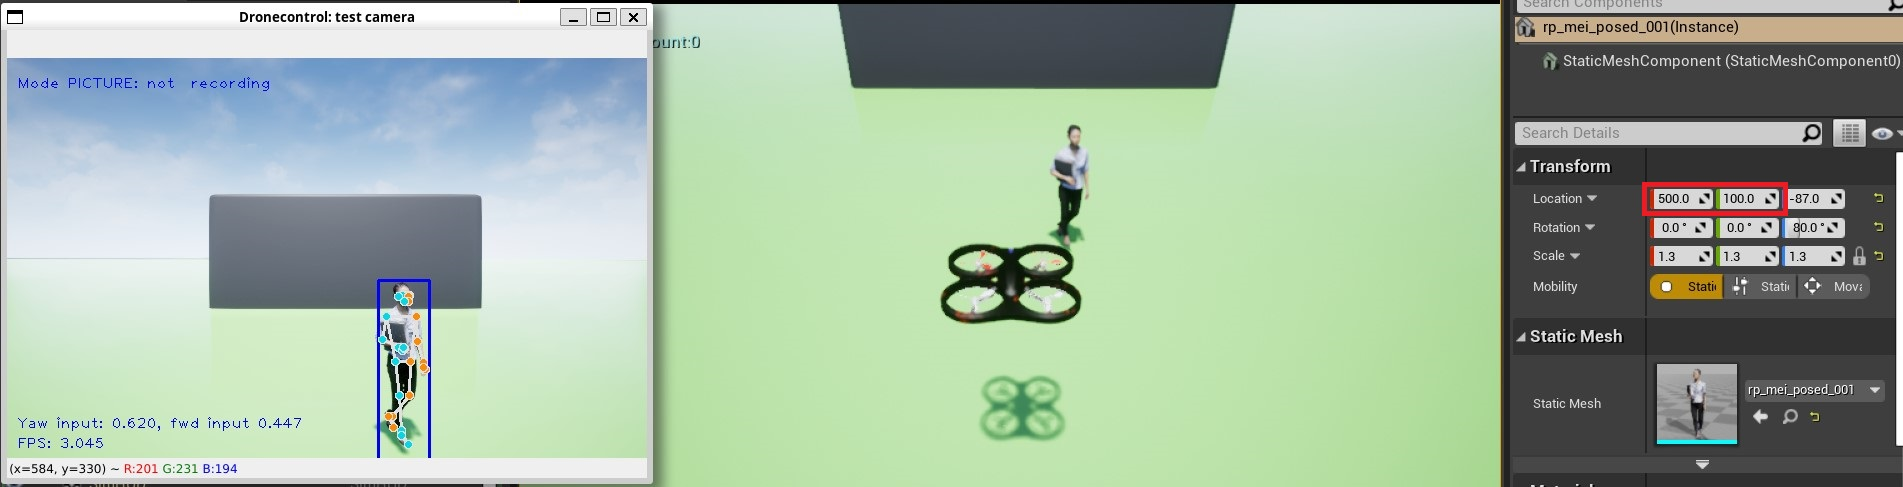
\includegraphics[width=\textwidth, keepaspectratio]{img/pid/tune-ref-pos-yaw.jpg}
  \caption{Starting position of the simulator for tuning the yaw controller. The human model is situated 500 units forward and 100 units to the right of the vehicle model.}
  \label{fig:tune-ref-pos-yaw}
\end{figure}


To tune the controller to its correct coefficients, the initial step will be testing different values of $K_{P}$ while keeping $K_{I}$ and $K_{D}$ at zero. Figure \ref{fig:tune-yaw-prop} displays the results of executing the tuning program for the five tested values of $K_{P}$, which range from $K_{P}=-10$ to $K_{P}=-90$ in increments of 20.
The left graph of the figure represents the variation in the horizontal position detected by the camera during the first 30 seconds after activating the controller. The right graph illustrates the yaw velocity outputted by the controller to the pilot module in order to reach the target.


\begin{figure}
  \centering
  \makebox[\textwidth][c]{
  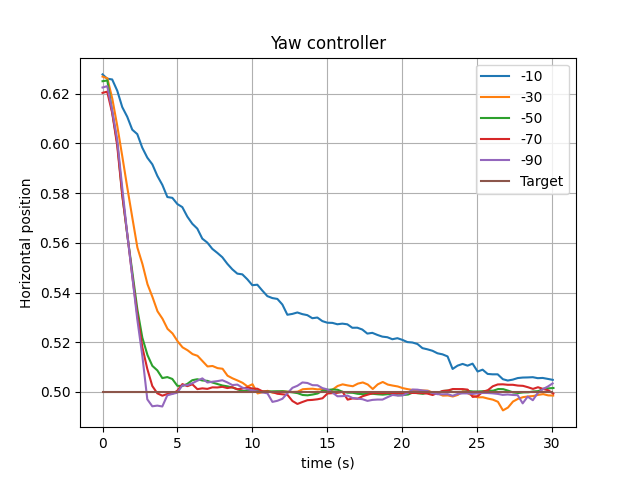
\includegraphics[width=.52\textwidth]{img/pid/yaw/yaw_pos_prop_i0_d0.png}
  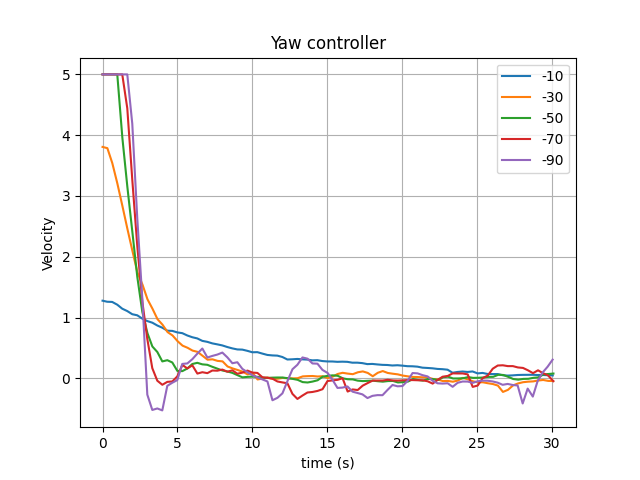
\includegraphics[width=.52\textwidth]{img/pid/yaw/yaw_vel_prop_i0_d0.png}}
  \caption{Variation of (a) input position and (b) output velocity for different values of $K_{P}$ and $K_I=0$, $K_D=0$ while the yaw controller is engaged.}\label{fig:tune-yaw-prop}
\end{figure}


For low values of $K_{P}$, the controller causes the vehicle to move slowly towards the target, resulting in a longer time to reach the midpoint position. Conversely, for high values of $K_{P}$, the controller attempts to rapidly approach the target, leading to oscillations around the target when it gets close. It is worth noting that the right graph demonstrates how the output velocity of the yaw controller is limited to 5 degrees per second. Thus, even with very high values of $K_{P}$, the vehicle will not rotate faster than this limit.

From the graphs, it can be observed that the most optimal value among those tested is $K_{P}=50$. At this value, the distance to the target point decreases rapidly (left graph), while the velocity does not exhibit significant fluctuations around zero (right graph).

The second step involves finding the correct value for $K_{I}$. To accomplish this, multiple values of $K_{I}$ will be tested while keeping $K_{P}$ at a low value of -20 and $K_{D}$ at 0. This setup allows for easier observation of the impact of the integral part on the controller.

Figure \ref{fig:tune-yaw-int-20} illustrates the behaviour of the input and output of the controller for a sample time of 40 seconds for each tested value of $K_{I}$. When $K_{I}=-1$, progress towards the target is stable and slightly faster compared to when the integral part is not contributing. However, as the magnitude of $K_{I}$ increases, noticeable oscillations around the target position emerge initially, then gradually diminish over time. For very large values of $K_{I}$, approximately from $K_{I}=-10$ in this case, the vehicle's velocity becomes locally unstable with numerous slight variations in its oscillations.

\begin{figure}
  \centering
  \makebox[\textwidth][c]{
  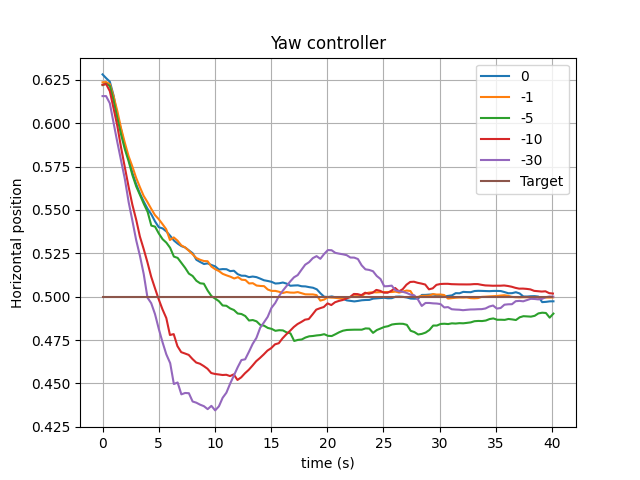
\includegraphics[width=.52\linewidth]{img/pid/yaw/yaw_pos_p20_int_d0.png}
  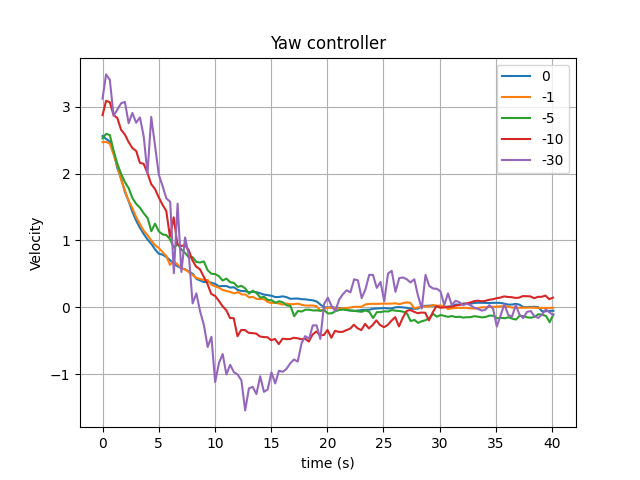
\includegraphics[width=.52\linewidth]{img/pid/yaw/yaw_vel_p20_int_d0.png}}
  \caption{Variation of (a) input position and (b) output velocity for different values of $K_{I}$ and $K_P=-20$, $K_D=0$ while the yaw controller is engaged.}\label{fig:tune-yaw-int-20}
\end{figure}

A similar effect can be observed to a lesser extent in Figure \ref{fig:tune-yaw-int-50}, where measurements were taken for $K_{P}=-50$ and $K_{D}=0$. In this graph, with $K_{I}=-1$, the controller reaches the target position approximately 3 seconds faster, exhibiting similar oscillations in velocity compared to exclusively using of the proportional term (Figure \ref{fig:tune-yaw-prop}, for $K_{P}=-50$).

\begin{figure}
  \centering
  \makebox[\textwidth][c]{
  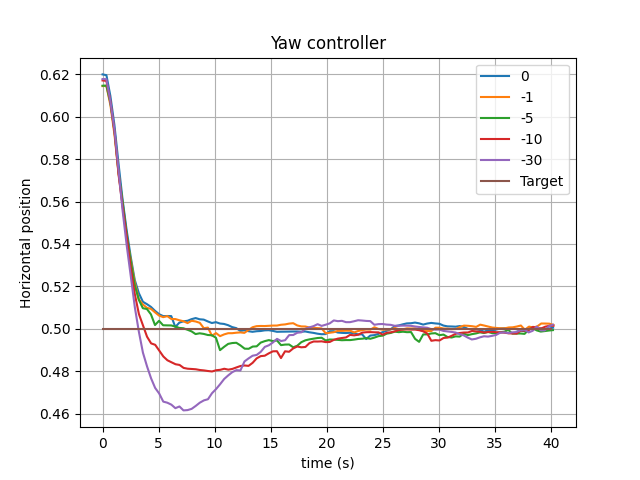
\includegraphics[width=.52\linewidth]{img/pid/yaw/yaw_pos_p50_int_d0.png}
  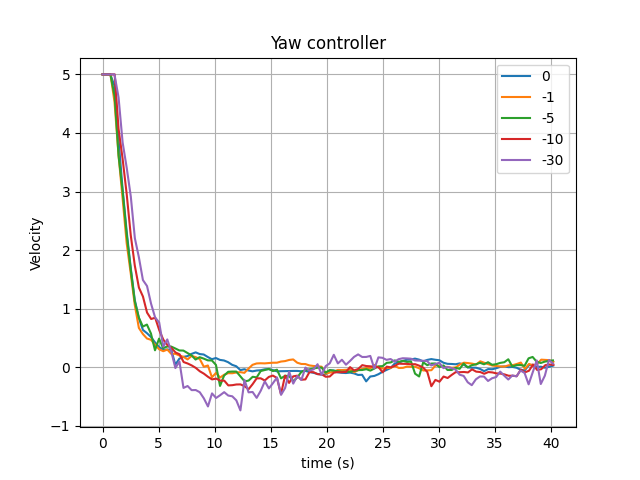
\includegraphics[width=.52\linewidth]{img/pid/yaw/yaw_vel_p50_int_d0.png}}
  \caption{Variation of (a) input position and (b) output velocity for different values of $K_{I}$ and $K_P=-50$, $K_D=0$ while the yaw controller is engaged.}\label{fig:tune-yaw-int-50}
\end{figure}


In the final step, the tuning process focuses on the derivative part of the controller. Multiple values of $K_D$ have been tested in conjunction with the chosen $K_P=-50$, both without any integral part ($K_I=0$) and with $K_I=-1$.
This combination aims to determine the impact of the derivative part on the controller and verify whether the integral part chosen in the previous step can work alongside it to enhance the controller's response to a changing input.

Figures \ref{fig:tune-yaw-der-i0} and \ref{fig:tune-yaw-der-i1} depict the evolution of the position detected by the computer vision system and the velocity outputted by the controller for a sample time of 40 seconds. Figure \ref{fig:tune-yaw-der-i0} corresponds to the case where $K_I=0$, while Figure \ref{fig:tune-yaw-der-i1} represents the case with $K_I=-1$, both with $K_P=-50$.

In all the tested scenarios, the iteration with $K_I=-1$ (Figure \ref{fig:tune-yaw-der-i1}) demonstrates better convergence towards the target positions compared to their respective $K_D$ values for $K_I=0$. This indicates that the integral part has been appropriately chosen. Moreover, it is worth noting that adding any amount to the derivative part does not yield any visible benefit in the step response of the controller. The curve that stabilizes first on the target position is still the one with $K_D=0$. Additionally, the velocity graph produces very similar results between $K_D=0$ and $K_D=-5$.

\begin{figure}[H]
  \centering
  \makebox[\textwidth][c]{
  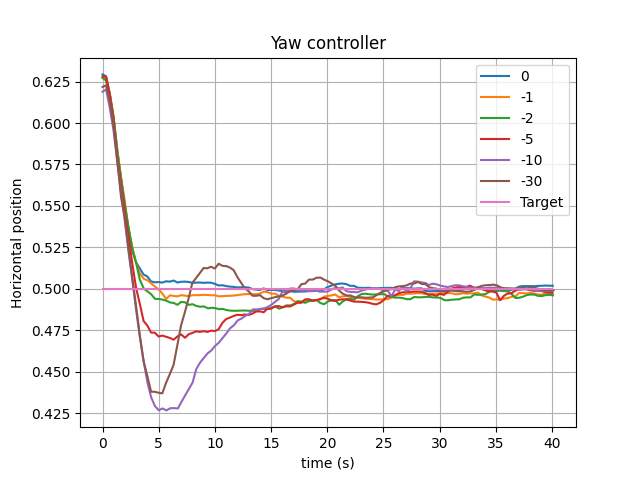
\includegraphics[width=.52\linewidth]{img/pid/yaw/yaw_pos_p50_i0_der.png}
  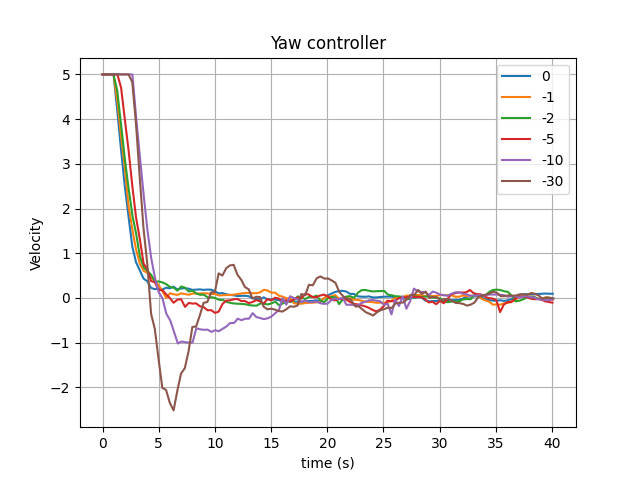
\includegraphics[width=.52\linewidth]{img/pid/yaw/yaw_vel_p50_i0_der.png}}
  \caption{Variation of (a) input position and (b) output velocity for different values of $K_{D}$ and $K_P=-50$, $K_I=0$ while the yaw controller is engaged.}\label{fig:tune-yaw-der-i0}
\end{figure}

\begin{figure}[H]
  \centering
  \makebox[\textwidth][c]{
  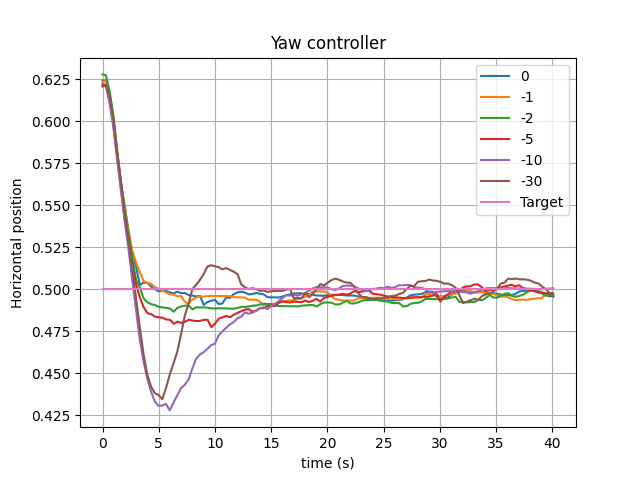
\includegraphics[width=.52\linewidth]{img/pid/yaw/yaw_pos_p50_i1_der.png}
  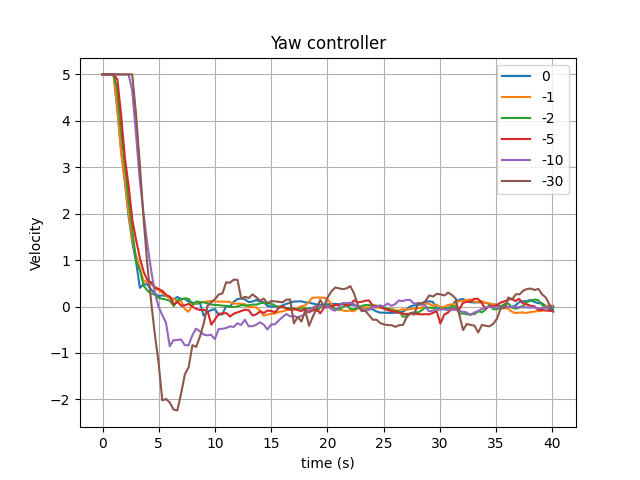
\includegraphics[width=.52\linewidth]{img/pid/yaw/yaw_vel_p50_i1_der.png}}
  \caption{Variation of (a) input position and (b) output velocity for different values of $K_{D}$ and $K_P=-50$, $K_I=-1$ while the yaw controller is engaged.}\label{fig:tune-yaw-der-i1}
\end{figure}

Based on these observations, the final coefficients for the yaw controller will be determined as $K_P=-50$, $K_I=-1$, and $K_D=0$. Consequently, the controller will effectively function as a PI (proportional-integral) controller rather than a complete PID (proportional-integral-derivative) controller. A recording of the whole tuning process for the yaw controller can be seen in this \href{https://l-gonz.github.io/tfg-giaa-dronecontrol/videos/tune-yaw-controller}{video}\footnote{\url{https://l-gonz.github.io/tfg-giaa-dronecontrol/videos/tune-yaw-controller}}.


\subsection{Forward controller}

The tuning process for the forward controller follows a similar procedure as the one used for the yaw controller. The initial setup for tuning involves positioning the figure closer to the vehicle than the reference position and ensuring it is centered in the vehicle's field of view. Figure \ref{fig:tune-ref-pos-fwd} illustrates this starting configuration, with the figure located at the (450,0) position in the simulated world. 

At this position, the input to the forward controller is 0.47, indicating that the bounding box around the detected figure occupies 47\% of the camera's field of view height. Consequently, the controller's response should be a negative forward velocity that moves the vehicle away from the target person, thereby reducing the perceived figure height. Since a negative output velocity directly reduces the input at the entrance of the controller, the coefficients for this PID controller should be positive. This is in contrast to the yaw controller, where the feedback loop was inversely proportional (a positive velocity decreased the input to the yaw controller).


\begin{figure}
  \centering
  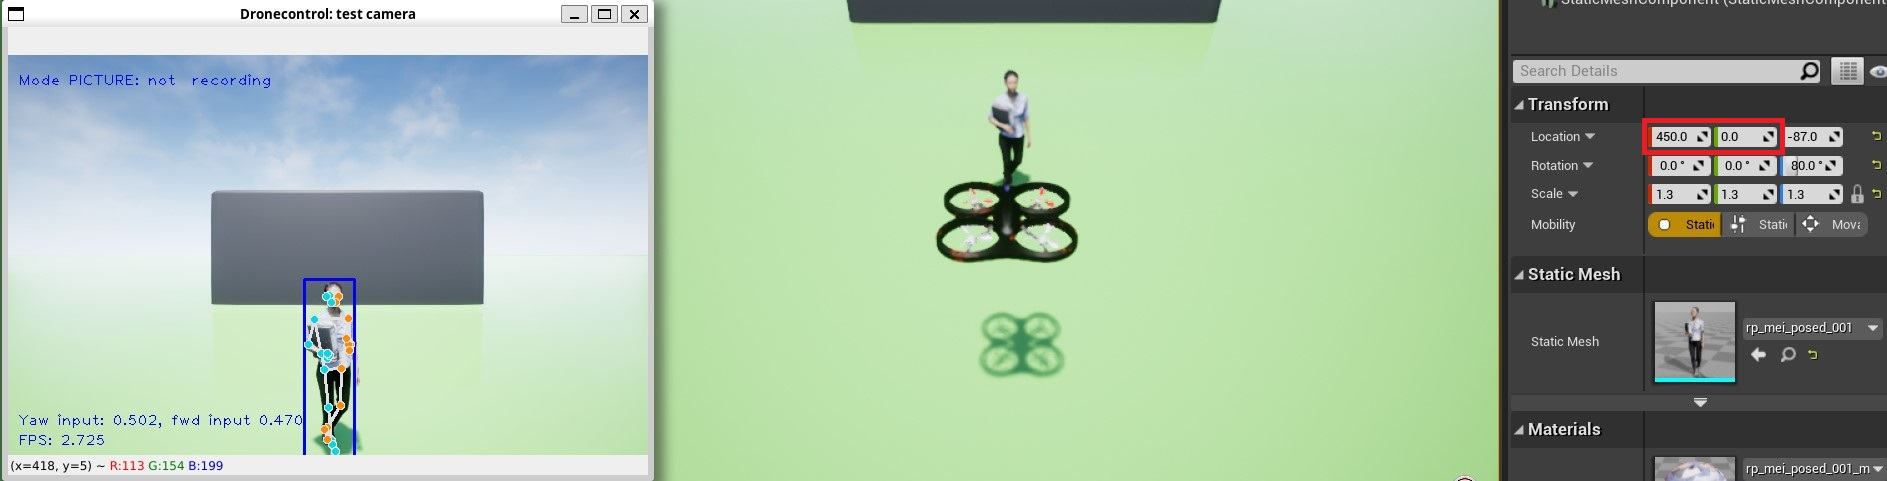
\includegraphics[width=\textwidth, keepaspectratio]{img/pid/tune-ref-pos-fwd.jpg}
  \caption{Starting position of the simulator for tuning the forward controller. The human model is situated 450 units forward and centred from the vehicle position.}\label{fig:tune-ref-pos-fwd}
\end{figure}


To begin the tuning process for the forward controller, the starting coefficients should be selected as it was done with the yaw controller. However, in this case, the forward velocity needs to be smaller than the yaw velocity to prevent destabilization of the camera caused by rapic pitch angle changes induced by the forward movement. Therefore, the coefficients to test for the forward controller will be reduced by one order of magnitude compared to the yaw controller.

Initially, values ranging from $K_P=1$ to $K_P=9$ in increments of 2 are tested, with $K_I=0$ and $K_D=0$, for a sample time of 30 seconds. The resulting curves generated by the controller for these coefficients are shown in Figure \ref{fig:tune-fwd-prop}. It is observed that the forward controller is generally more unstable compared to the yaw controller due to the influence that fast forward and backward movements have on the pose detection algorithm.

This is particularly visible at the start of each test as slightly different heights are detected in the image from the camera even though the vehicle is in the same position relative to the human figure. The high sensitivity of the detection mechanism creates an aditional effect, especially for the bigger $K_P$ values tested. As the vehicle begins its movement back to the target position, the pose detection mechanism captures a slightly different perspective of the followed person, leading to increases in the detected height. This increase is reflected in the small spikes at the beginning of the detected height graph on Figure \ref{fig:tune-fwd-prop}, despite the fact that the velocity graph shows a negative velocity, indicating that the vehicle is moving backward away from the person.

To mitigate this effect, it is important to keep the output forward velocity small in the controller. The right graph of Figure \ref{fig:tune-fwd-prop} also demonstrates that for high values of $K_P$, the output velocity increases significantly, reaching the maximum velocity limit of \unitfrac[0.4]{m}{s} set for the forward controller. A value of $K_P$ up to 3 provides a rapid descent without significant oscillations around the target height, making it a suitable choice for the final controller.


\begin{figure}[H]
  \centering
  \makebox[\textwidth][c]{
  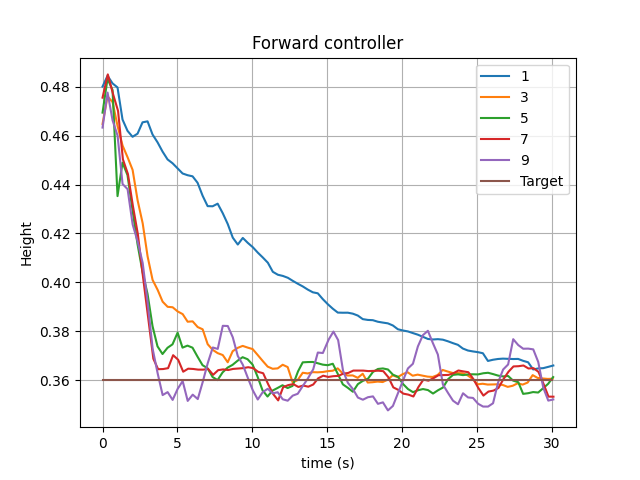
\includegraphics[width=.52\linewidth]{img/pid/fwd/aaa_fwd_pos_prop_i0_d0.png}
  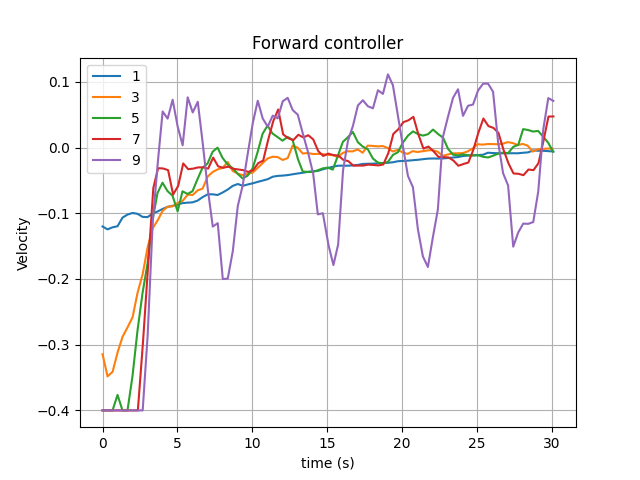
\includegraphics[width=.52\linewidth]{img/pid/fwd/aaa_fwd_vel_prop_i0_d0.png}}
  \caption{Variation of (a) input height and (b) output velocity for different values of $K_{P}$ and $K_I=0$, $K_D=0$ while the forward controller is engaged.}\label{fig:tune-fwd-prop}
\end{figure}


The tests for $K_I$ and $K_D$ in the forward controller are depicted in Figures \ref{fig:tune-fwd-int} and \ref{fig:tune-fwd-der}, respectively. Increasing the coefficient for the integral part leads to initial overshooting of the target position, followed by stabilization and approximation to the target. However, since overshooting is not desirable in this application due to safety concerns, a value of $K_I=0$ is chosen for the forward controller. 

In the case of the derivative component, all tested values of $K_D$ lead to increased oscillations in the system. Therefore, it is decided to exclude the derivative part from the forward controller. As a result, the final coefficients for the forward controller will be $K_P=3$, $K_I=0$, and $K_D=0$, making it simply a proportional controller without integral or derivative components.

\todo[inline]{Rerun with Kp = 3 ?????}
\begin{figure}[H]
  \centering
  \makebox[\textwidth][c]{
  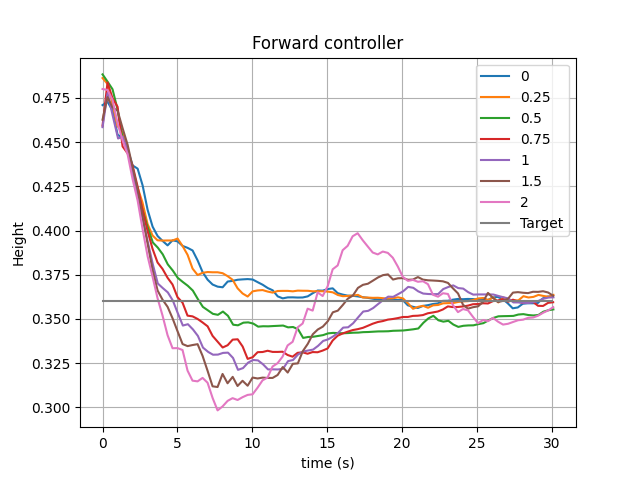
\includegraphics[width=.52\linewidth]{img/pid/fwd/aaa_fwd_pos_p3_int_d0.png}
  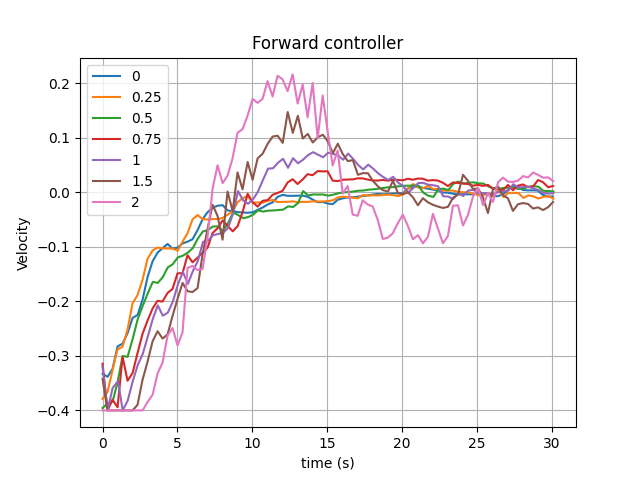
\includegraphics[width=.52\linewidth]{img/pid/fwd/aaa_fwd_vel_p3_int_d0.png}}
  \caption{Variation of (a) input height and (b) output velocity for different values of $K_{I}$ and $K_P=7$, $K_D=0$ while the forward controller is engaged.}\label{fig:tune-fwd-int}
\end{figure}
\begin{figure}[H]
  \centering
  \makebox[\textwidth][c]{
  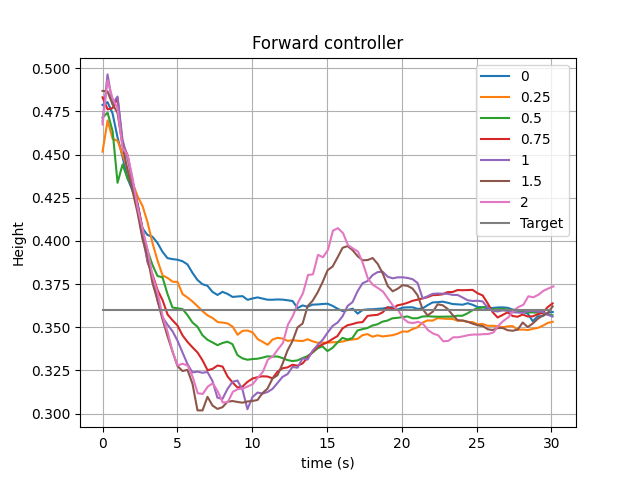
\includegraphics[width=.52\linewidth]{img/pid/fwd/aaa_fwd_pos_p3_i0_der.png}
  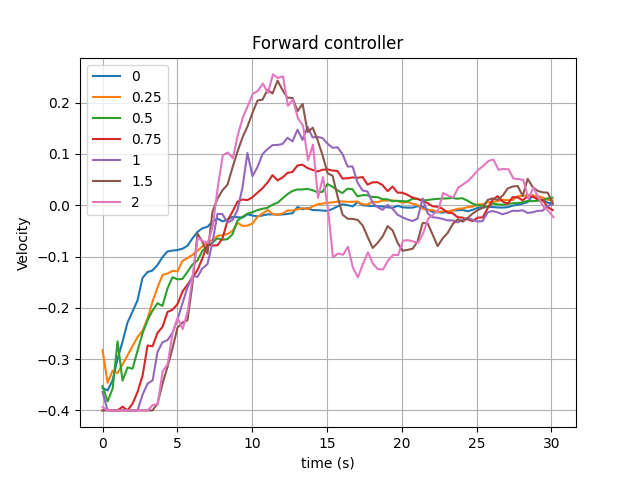
\includegraphics[width=.52\linewidth]{img/pid/fwd/aaa_fwd_vel_p3_i0_der.png}}
  \caption{Variation of (a) input height and (b) output velocity for different values of $K_{D}$ and $K_P=7$, $K_I=0.5$ while the forward controller is engaged.}\label{fig:tune-fwd-der}
\end{figure}


\subsection{PID tuning validation}
\label{subsec:pid-test-controller}

The final validation of the tuning obtained for the controllers will be performed using the \texttt{test-controller} tool described in Section \ref{subsec:pid-tools}. The goal is to check the step response of the controllers for different starting distances and validate their performance when engaged simultaneously. For the first test, the starting distances will vary along the y-axis, and for the second one, they will vary along the x-axis.

In the first test, the positions will vary along the y-axis, meaning that the figure will move from left to right in the field of view of the vehicle. The y-coordinates to be tested will range from -150 to 150 units in increments of 50, while the x-coordinate of the figure in the simulated world will remain fixed at $x=500$.

The results of the first run are shown in Figure \ref{fig:validate-yaw}. The y-coordinates tested range from -150 to 150 units in increments of 50, while the x-coordinate of the figure in the simulated world remains fixed at $x=500$. These changes in position mean that the figure moves from left to right in the field of view of the vehicle, following a line parallel to the lateral axis of the vehicle. To counteract this movement, both the yaw and forward controllers need to engage to reach the reference position.

The plots in Figure \ref{fig:validate-yaw} depict the changes in the normalized horizontal distance and normalized figure height detected by the person recognition algorithm during the time it takes for the vehicle to reach the target distance from the human figure for each tested start position. The target is considered reached when the error is less than 2\% and the output speed at the controller is less than 10\% of the maximum value. The full execution of the \texttt{test-controller} tool with varying lateral positions can be seen in the video found in the project's \href{https://l-gonz.github.io/tfg-giaa-dronecontrol/videos/test-yaw-controller}{page}\footnote{\url{https://l-gonz.github.io/tfg-giaa-dronecontrol/videos/test-yaw-controller}}.

\begin{figure}[H]
  \centering
  \makebox[\textwidth][c]{
  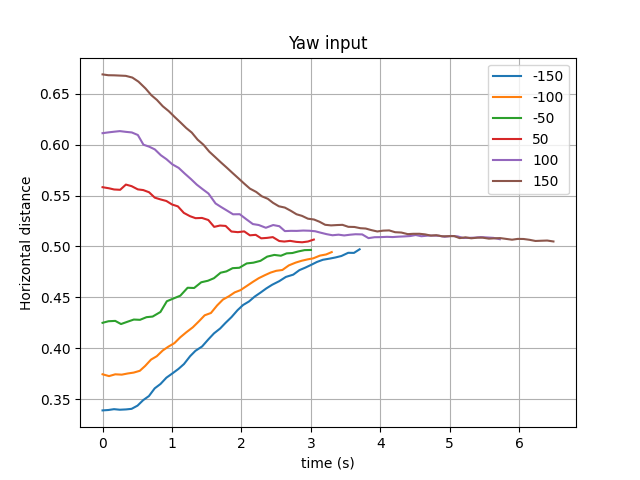
\includegraphics[width=.52\linewidth]{img/pid/validation_yaw.png}
  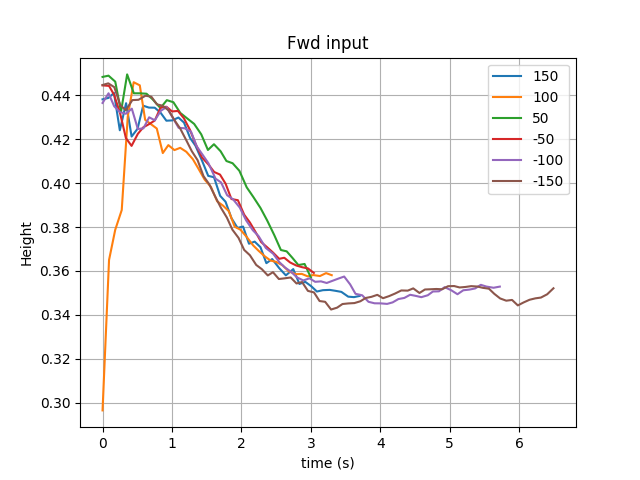
\includegraphics[width=.52\linewidth]{img/pid/validation_yaw_2.png}}
  \caption{Changes over time in detected horizontal position and height as input for the controllers with different starting positions in the y-axis}
  \label{fig:validate-yaw}
\end{figure}

During execution, the yaw controller introduces a negative yaw velocity when the figure is on the left half of the camera's field of view and a positive yaw velocity when the figure is on the right half, aiming to achieve a target horizontal distance of 0.5 (centred in the camera image). On the other hand, the forward controller outputs a negative forward velocity to reduce the detected height of the figure from around 0.44 to the target value of 0.36.

Looking at Figure \ref{fig:validate-yaw}a, it can be observed that most of the time is spent initiating the movement towards the target. Once the vehicle starts moving, there is not much difference between the -50 and the -150 steps in the time it takes to reach the target position, with the former taking around 3 seconds and the latter taking approximately 3.6 seconds. 

In Figure \ref{fig:validate-yaw}b, the trajectories appear quite similar since the starting distance to the target is the same for all the cases. For each run, the controller guides the vehicle to move backwards, ensuring that the figure stays sufficiently far away, resulting in a decrease in the detected height. Additionally, a detection anomaly can be observed in Figure \ref{fig:validate-yaw}b. For the starting position at $y=100$ (yellow line), there is a brief initial period where the detected height is very small due to a detection error in the first frames processed by the computer vision algorithm. However, within half a second, the detection stabilizes, and the controller successfully guides the vehicle to the target position without significantly impacting the time taken or the final position. This demonstrates that the controllers are capable of recovering from detection errors without compromising the vehicle's movement.


\begin{figure}[H]
  \centering
  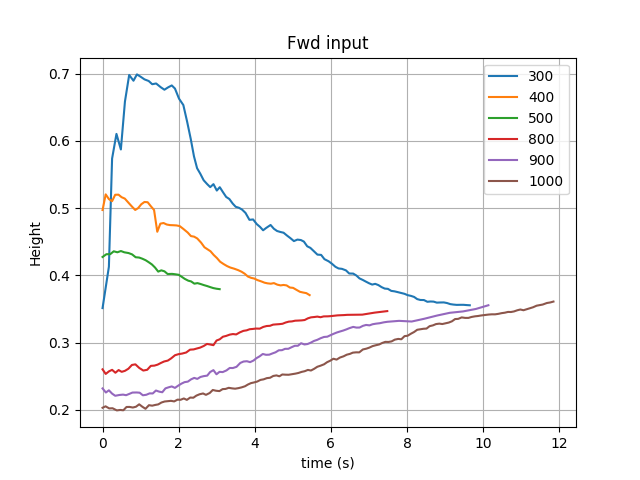
\includegraphics[width=.7\textwidth, keepaspectratio]{img/pid/validation_fwd.png}
  \caption{Changes over time in detected height as input for the forward controller with different starting positions in the x-axis}
  \label{fig:validate-fwd}
\end{figure}


To further validate the performance of the forward controller, the \texttt{test-controller} tool can be used with varying positions along the x-axis. This means that the tests are conducted with the human figure at different distances along the longitudinal axis of the vehicle, closer and further away than the reference distance. Throughout the process, the figure is kept centred in the camera's field of view (y position remains 0). Therefore, in this scenario, the yaw controller does not need to be considered.

Figure \ref{fig:validate-fwd} illustrates the changes over time in the input to the forward controller for each starting position as the vehicle moves towards the target position. The graph highlights significant differences in how the controller responds to positions closer or further away from the target distance. When the person is very close to the vehicle, there are substantial differences in detected heights for minor changes in longitudinal distance, leading to the rapid movement of the vehicle away from its start position. Conversely, when the person is further away from the vehicle than the target, the same differences in distance are associated with minor differences in detected height. As a result, the controller determines a smaller velocity output compared to the cases when the person is closer to the vehicle. Consequently, it takes a longer time for the vehicle to reach the target position.

Notably, even when the person is so close to the vehicle that part of their figure falls outside the camera's field of view, the pose detection mechanism functions well enough to estimate the person's continued position outside the image. This can be seen on Figure \ref{fig:validate-fwd} for the case of $x=300$, where the detected height starts lower than it should be and gradually increases as the full person starts to fit in the camera's field of view.
\\ \\


\begin{figure}[H]
  \centering
  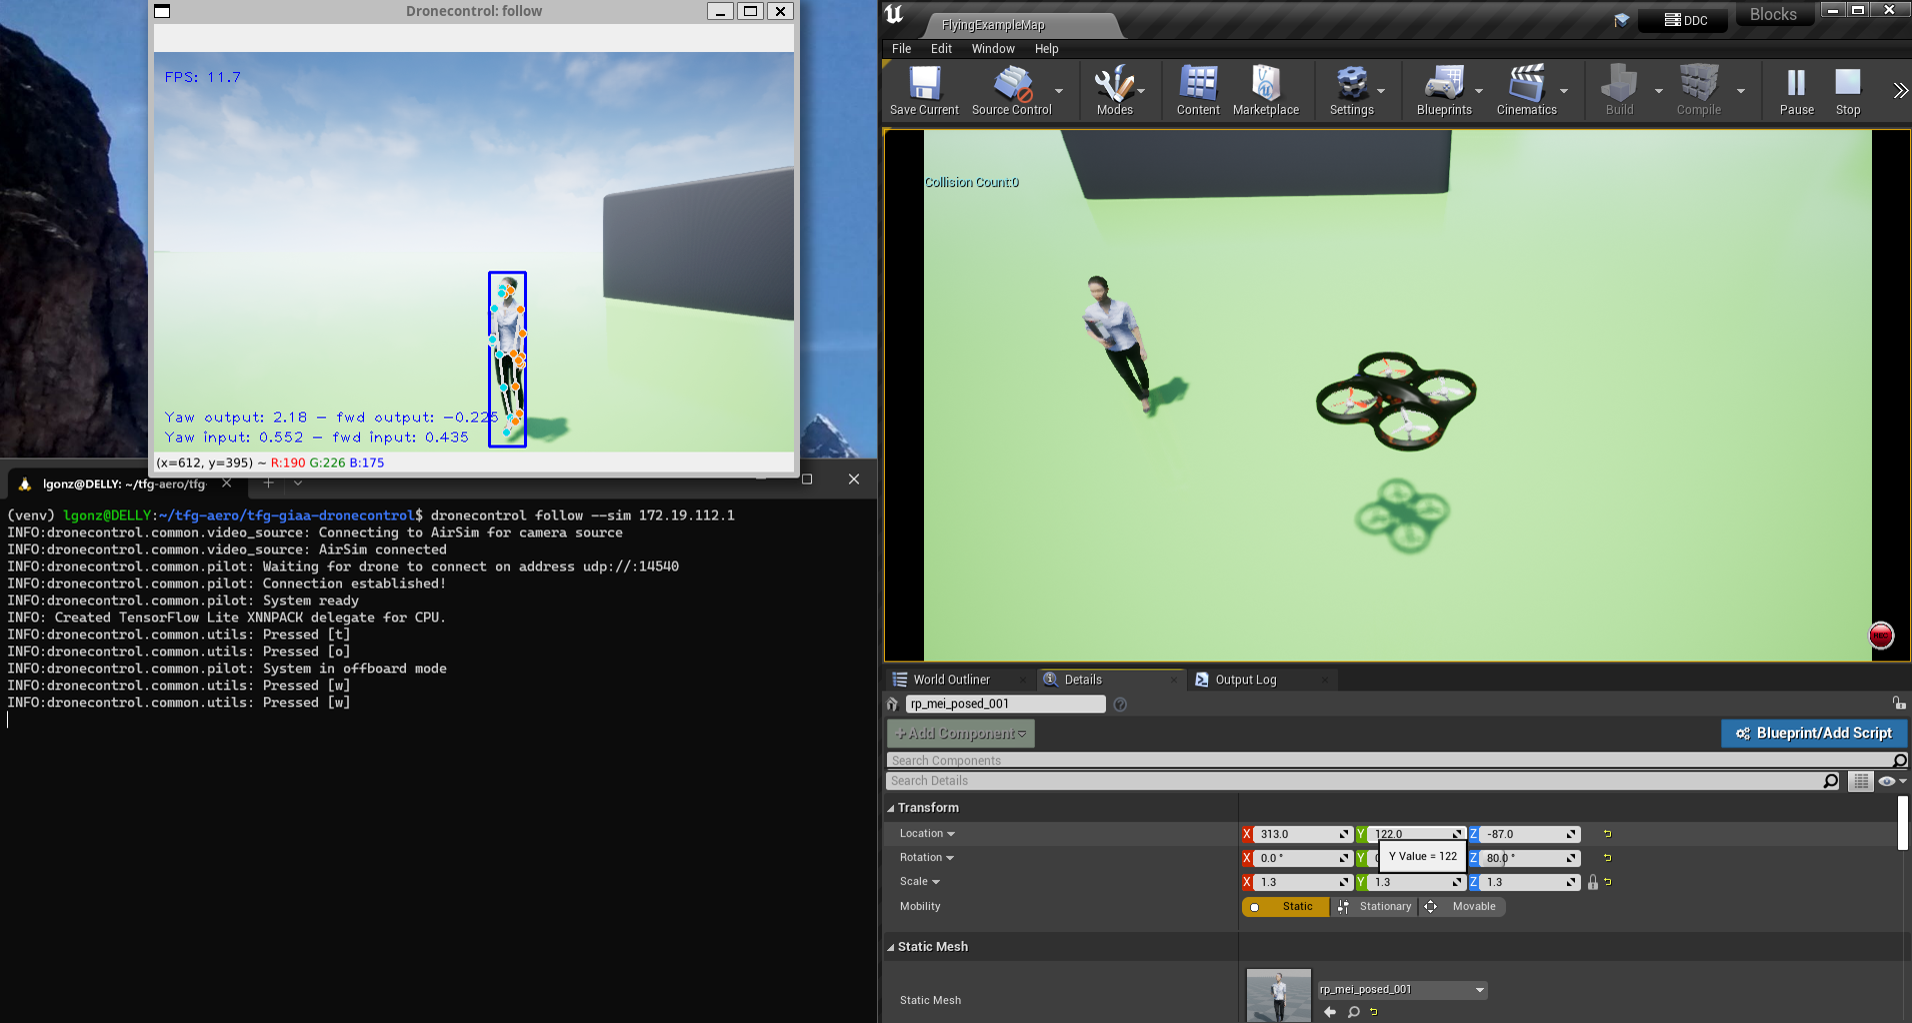
\includegraphics[width=\textwidth, keepaspectratio]{img/video-follow-sitl.png}
  \caption{Single frame from the video showing the movement of the drone in response to changes in the position of the tracked person}
  \label{fig:airsim-test-follow}
\end{figure}

Overall, the results of the validation process indicate that the tuned controllers perform effectively, and accurately follow the person across different starting positions, even when detection errors occur. They successfully respond to variations in the person's distance and angle from the vehicle, allowing for accurate tracking and movement towards the target relative position.

The selected coefficients for the controllers can now be applied to the complete follow solution in order to assess the expected performance of the vehicle in real flights. To provide a visual demonstration, a video showcasing the drone's movement using these parameter values can be accessed \href{https://l-gonz.github.io/tfg-giaa-dronecontrol/videos/test-sitl-follow}{here}\footnote{\url{https://l-gonz.github.io/tfg-giaa-dronecontrol/videos/test-sitl-follow}}. Additionally, Figure \ref{fig:airsim-test-follow} displays a frame extracted from the video, giving a glimpse of the drone's behaviour during the follow operation.



